%!TEX root = ../main.tex

\section{CAN Bus}
\label{sub:CAN_Bus_Tests}
With the CAN controller available on the PS of the Zybo, the CAN bus will be tested to determine the transmission abilities of the network.
The transceivers are able to work at up to 8 Mb/s, while the CAN controllers on the Zybo only guarantee functionality up to 1 Mb/s. 
As the final implementation might be done in PL, there is nothing preventing the controller working at 8 Mb/s -- the FPGA can easily produce and interpret signals up to or beyond 8 Mb/s.\\

The tests are performed using the block diagram from figure~\ref{fig:CAN_Testing_Architecture}, on page~\pageref{fig:CAN_Testing_Architecture} as the FPGA part, though not all parts of this block diagram is used for each part.
Software will be developed for bare metal purpose, and because of this, not all tests will be performed using interrupts, as the Zybo has no other task that it can be interrupted from.
\martin{@Catalin, I would like to keep the names short and descriptive}
The tests performed will be: 
\begin{itemize}
	\item \textbf{Basic communication}: Proving the ability for basic communication between nodes, while confirming, that the CAN stack works.
	\item \textbf{Latency tests}: Measuring the time it takes to send one large frame
	\item \textbf{Bandwidth}: Determining how much raw data can be transmitted per unit time
	\item \textbf{Priority when multiple node sending}: Ensuring, that higher message ID make way for the lower ones 
\end{itemize}

\subsection{Basic Communication}
\label{sub:TestingCANStack_BareMetal}
After the design and printing of the stack board, testing it was the next step.
The test included using one the CAN controllers within the Zynq chip with the purpose of showing that a basic CAN network between two Zybo boards could be implemented using the stack.
Specifically, the one Zybo was sending the input value of the buttons to the network in order to be received by the second one and turn on the appropriate on-board LEDs as a result.
After programming the FPGA with the basic architecture designed in Vivado as seen in figure \ref{fig:CAN_Testing_Architecture} and uploading the source code written in Vivado SDK, the test was successful, thus proving the basic functionality of a CAN network.
The messages sent from the first node to the second one were received correctly, containing the intended value of the buttons.
A two-way communication was also proven, since both boards had a SendFrame() and a RecvFrame() function (common source code), thus one controlling the LEDs of the other one.
The test was successful with more than two Zybo boards as well, proving the ability to create a network of multiple nodes communicating with each other.
In the last case, the button values sent from one node were received by all the other nodes turning on the same LEDs.
All Zybo boards were programmed with the same architecture and source code.

\subsection{Latency Test}\label{sub:CAN_latency}
For this test, only two Zybos are needed.
One node prepares a frame for transmission, then sets a GPIO pin high.
It then performs the necessary checks and writes the message details to the TX fifo, and then sets its GPIO pin low. \\
The other node will then wait for the full message frame to be received, and then set its GPIO pin high.
Once the metadata of the message (data length and message ID) has been intepreted, the voltage goes low again.
Using an oscilloscope, it is possible to measure the time it takes to send a message.\\

The test will be performed for an 8 byte frame.
The messages will be constructed, so that bit stuffing doesn't occur by writing 0xA1 to 0xA8. 
The resulting voltage measurements are displayed on figure~\ref{fig:CAN_test1_raw}

\begin{figure}[h]
	\centering
	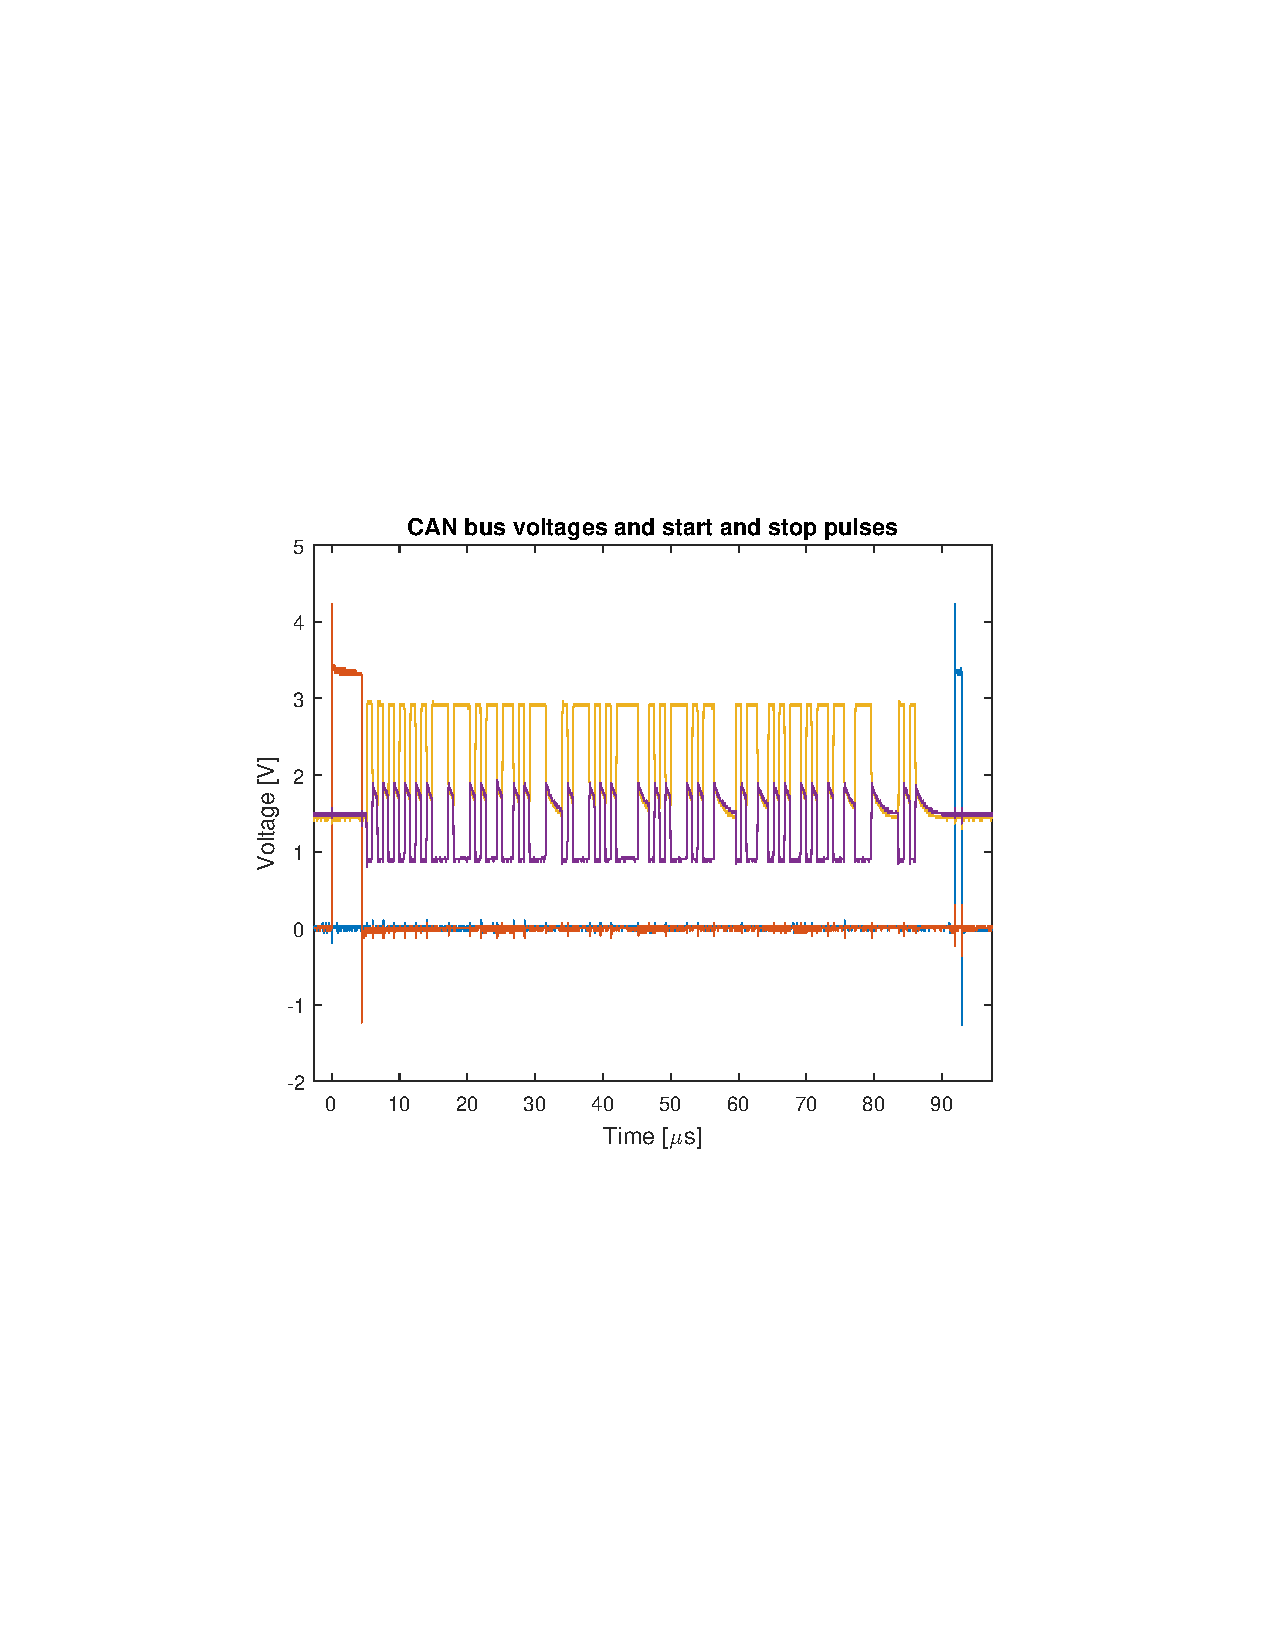
\includegraphics[width = \linewidth]{graphics/CAN_test1_raw}
	\caption{Start and stop pulses for an 8 byte CAN message}
	\label{fig:CAN_test1_raw}
\end{figure}

The time from the red voltage goes low, to the time the blue voltage goes high is $87.5 \si{\micro\second}$.
This is of course very dependent on the particular controller used for this test, which according to the datasheet can work up to 1 MHz.
Measuring this test shows, that pulses come at 1.25 MHz.
The software used for basis of this test does allow to adjust a pre-scaler, so that the controller works faster, but it is not able receive frames at a higher rate than 1.25 MHz.\\

The CAN bus voltage can be interpreted to bits, to show what's actually being transmitted.
This is done by measuring the voltage difference between the yellow and purple graphs, keeping in mind, that a difference in voltage corresponds to a zero, while no difference corresponds to a one.
The CAN frame is displayed and interpreted on figure~\ref{fig:CAN_test1_message}.

\begin{figure}[h]
	\centering
	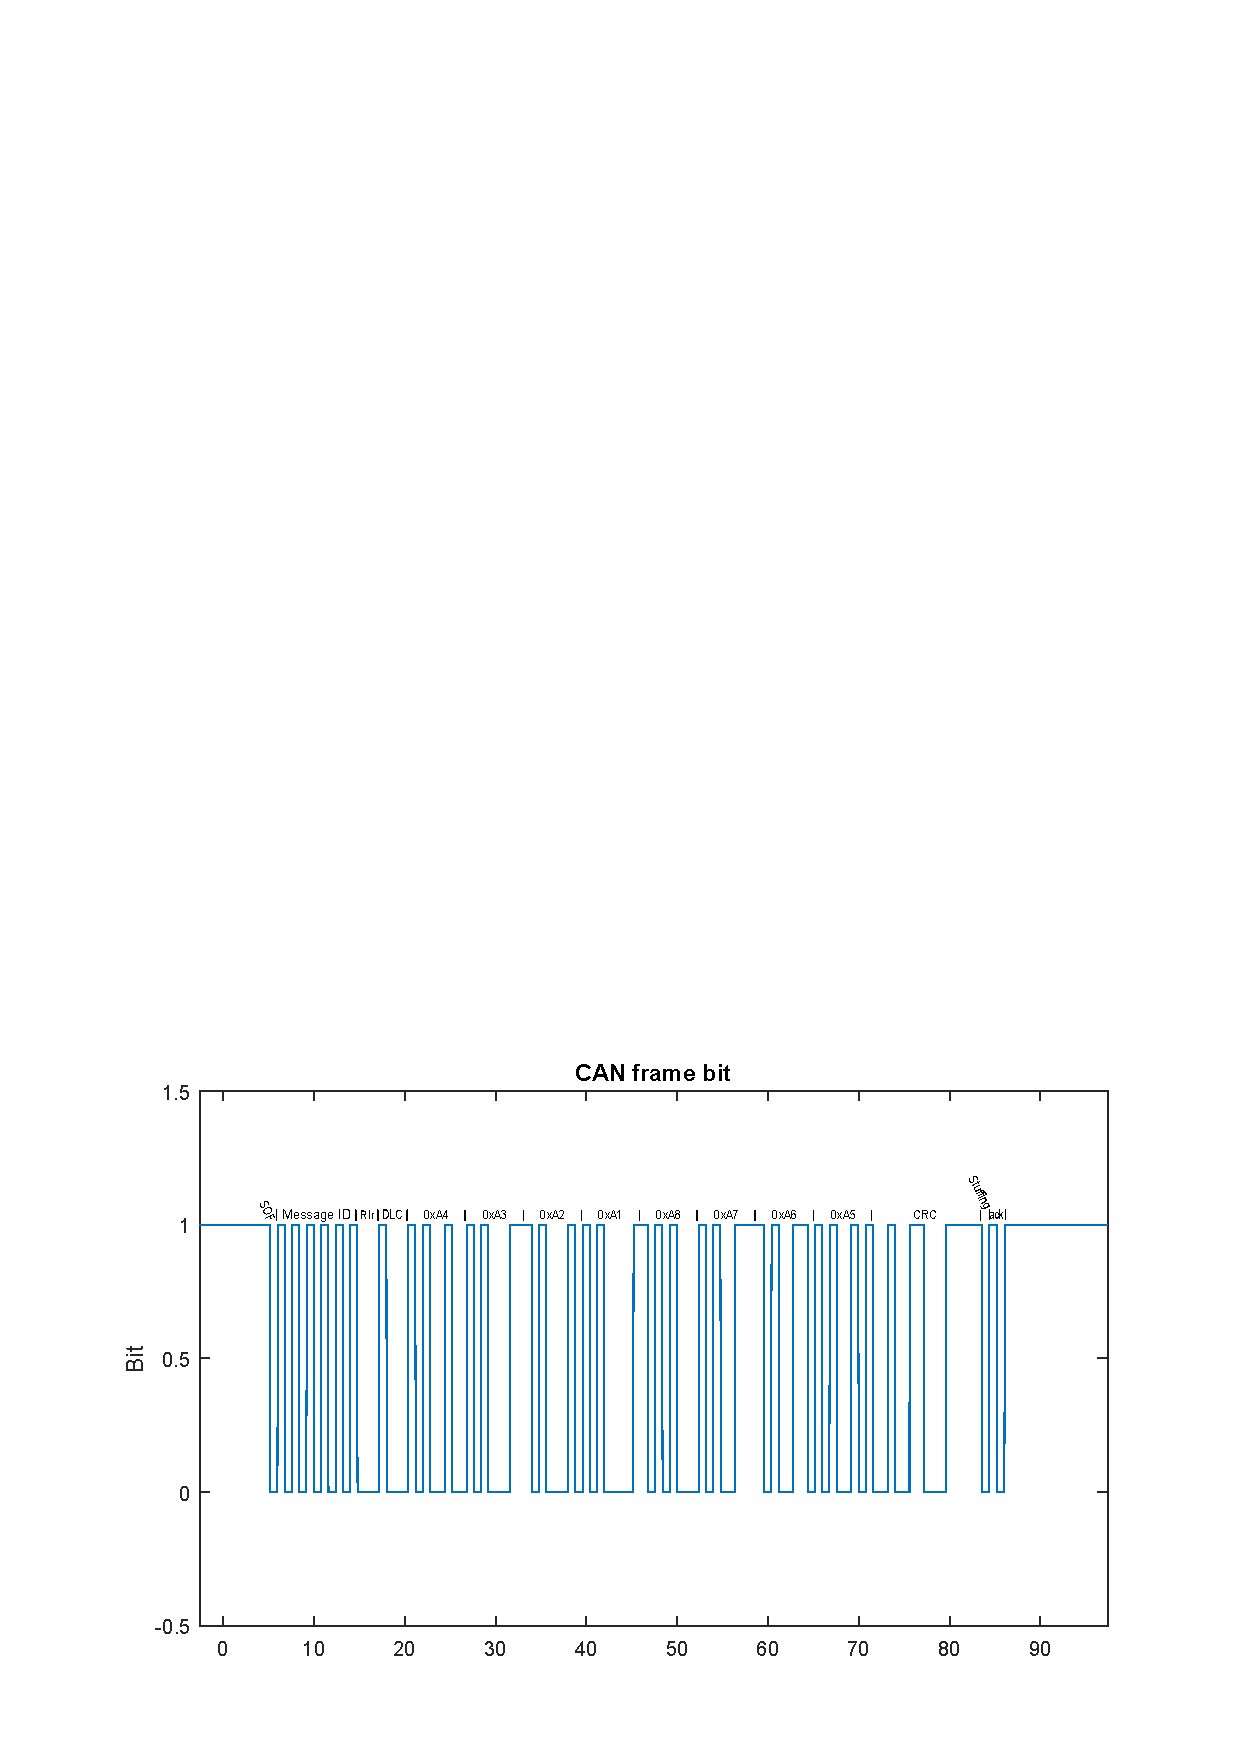
\includegraphics[width = \linewidth]{graphics/CAN_test1_message}
	\caption{Bit interpretation of the CAN frame. RIr  is the tree bits: RTR, ID Extention and r0, which are all 0.}
	\label{fig:CAN_test1_message}
\end{figure}

The data portion of the frame is bitwise big endian, but bytewise little endian. 
The message to be sent was codes as two 32 bit unsigned integers: 0xA1A2A3A4 and 0xA5A6A7A8.
The controller then swapped the bytes around, causing the data to become little endian.
This is a convention implemented by the CAN controller, and as the same endianness is applied when sending and receiving the frame, it doesn't matter -- the CAN bus does not care about the order bits in the data portion. 
The message was received correctly.\\

The CRC was calculated automatically by the controller.
Unfortunately it ends on five consecutive 1's, meaning that a 0 must be stuffed in-between the delimiter, causing the frame to be one bit longer.\\

Additionally this controller uses 5 bits for the IFS part of the frame, rather than the mandatory minimum of 3 bits. 



\subsection{Bandwidth}\label{sub:CAN_bandwidth}
This will be calculated, as the faster controllers are not available.
Bandwidth is considering the amount of net data being transmitted per unit time, when excluding the overhead.
Bandwidth will be calculated for 8 byte frames, and bit stuffing will be omitted.\\

The maximum operating data rate for the transceivers is 8 Mb/s.
As mentioned in section~\ref{sub:CanMessageFrame}, the CAN frame has 47 bits of overhead. 
Including 8 bytes of data, this comes up to 111 bits. 
Time per frame is:

\begin{equation}
\frac{111}{8 \cdot 10^6} = 1.39 \cdot 10^{-5}
\end{equation}

As each frame contains 8 bytes of data, the data rate becomes:

\begin{equation}
\frac{8}{1.39 \cdot 10^-5}= 5.77 \cdot 10^5
\end{equation}

That means, that the effective transfer rate is 577 kB/s, or 4.61 Mb/s with 8 Mb/s controllers. 
With the controllers built into the PS of the Zybo, this effective rate comes down to 720 kb/s.

\catalin{Explain how the test was done in terms of software. Also explain why GPIO interrupts were not suitable or used.}
\subsection{Message Priority}\label{sub:CAN_message priority}
This test is based on the CAN polled example, where two Zybos will transmit data.
The two transmitting Zybos will prepare a CAN frame with the same data content, but different message IDs.\\
Zybo A will send message ID 0b10100100000.\\
Zybo B will send massage ID 0b10101000000.\\
I.e. only the fifth and sixth bits have been swapped, meaning that Zybo A will have the higher priority.
Both of these Zybos will prepare their respective Tx frame, and continuously poll the PMOD port.
The PMOD connection must be configured to have pull down, to ensure that unconnected pins are set low.
Using a DC voltage source, this GPIO port of each Zybo will be set high simultaneously.\\

When the PMOD returns a non-zero value, each Zybo will call the XCanPs\_Send function twice.
This will fill two frames with 8 bytes of data into the Tx Fifo of each Zybo. 
Because of the asynchrous nature of the CAN protocol, it is still somewhat random which message gets transmitted first, so the frame will be sent twice. 
This means, that after the first frame is sent from either one of the Zybos, both zybos will start transmitting at the same time. 
In this case one Zybo must stop transmitting when it realizes that it has the lower priority.
This is shown on figure~\ref{fig:CAN_test3_2TX}.\\

\begin{figure}[h]
	\centering
	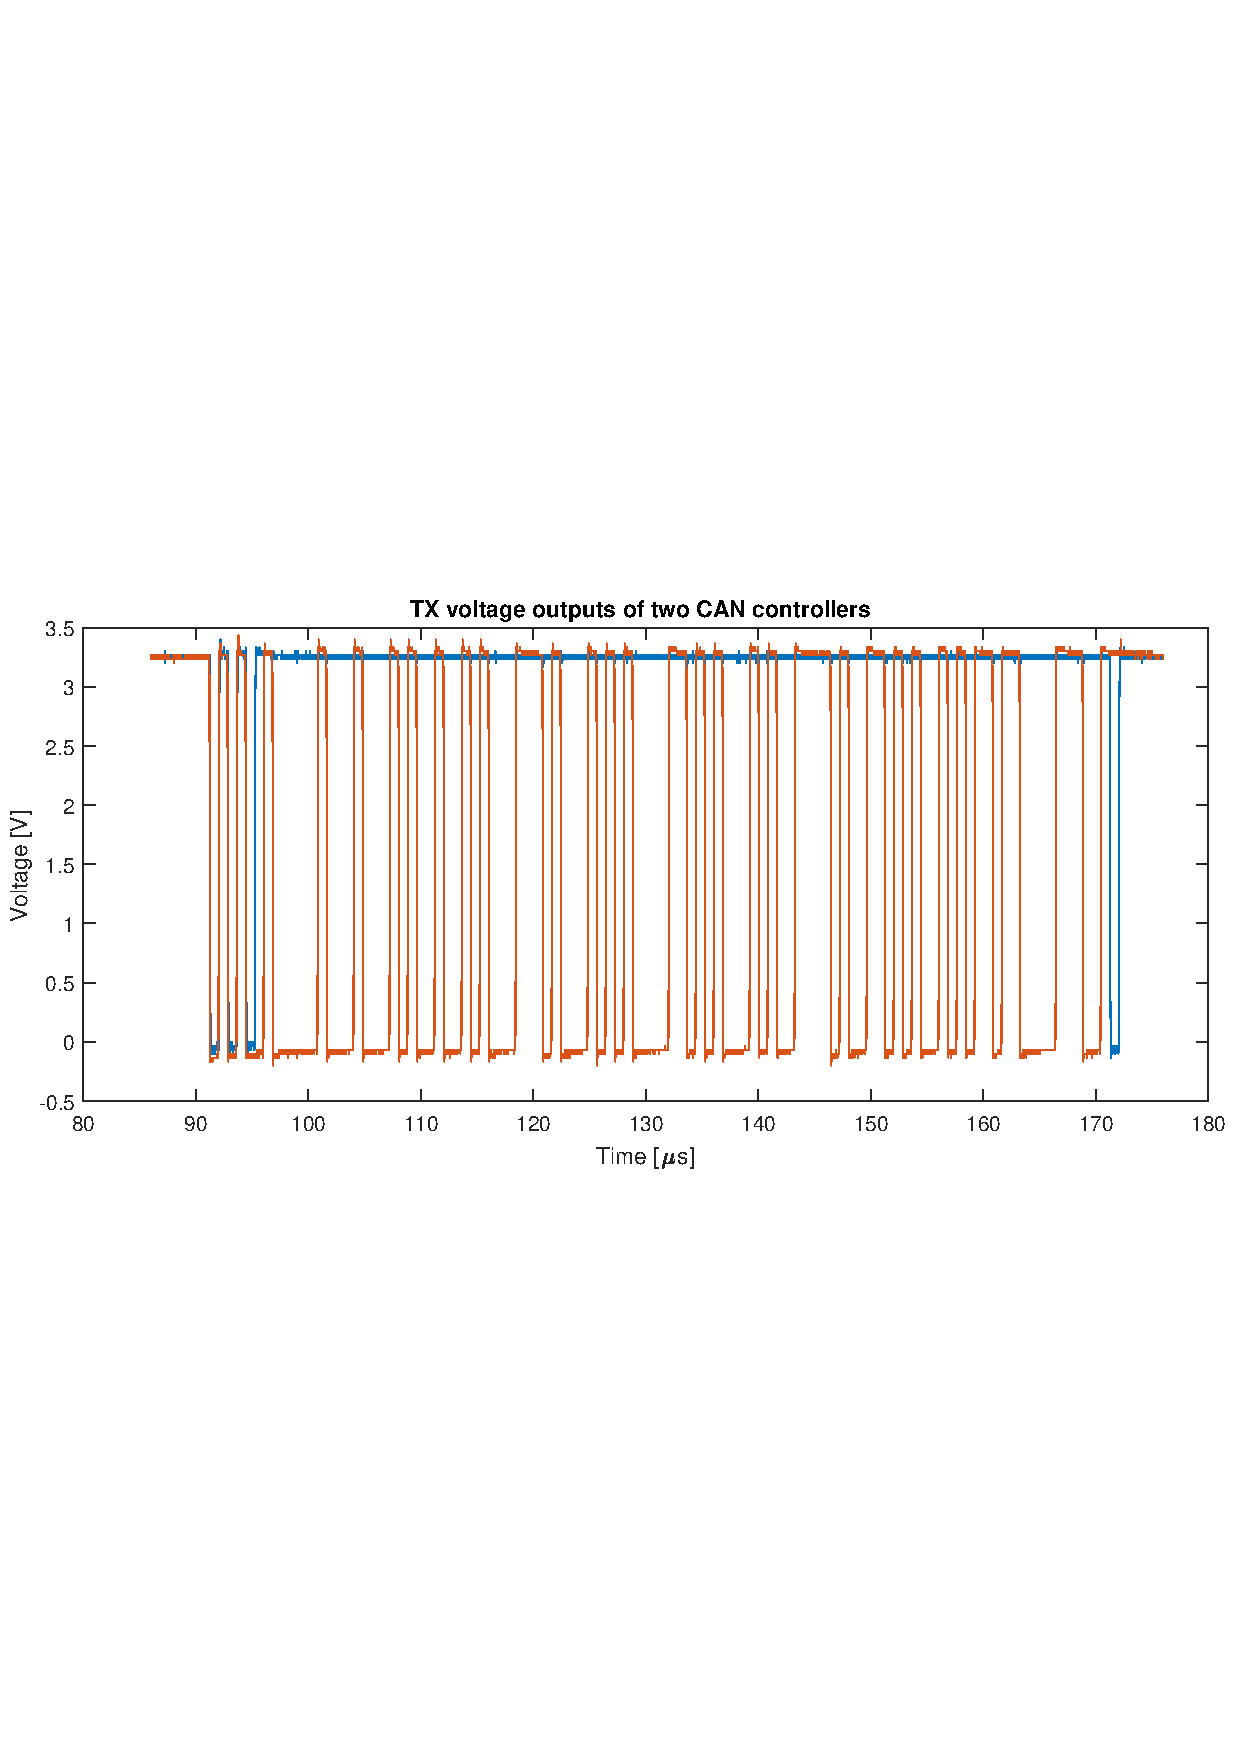
\includegraphics[width = \linewidth]{graphics/CAN_test3_2TX}
	\caption{Voltage measurements taken at the TX pin of Zybo A (red) and Zybo B (blue).}
	\label{fig:CAN_test3_2TX}
\end{figure}

The displayed frame is the second of four frames sent for this test, which is why the graph starts at $80 \si{\micro\second}$.
Both Zybos start sending their frame simultaneously, and as there is no difference until the fifth bit of the message ID, neither Zybo is aware that the other is also sending.
At the time $95.3\si{\micro\second}$, Zybo B (blue line on figure~\ref{fig:CAN_test3_2TX}) sends out high, whilst receiving low, meaning that another node is sending as well. 
It will then cancel this attempt to transmit, and wait until the current frame has been transmitted before it will try again.
Also note the Zybo B writing the acknowledge bit at the time $171 \si{\micro\second}$.
Because of this, it is not strictly necessary to use a receiving Zybo, because the other node will confirm the CRC of the message.\\

\subsection{Conclusion}\label{sub:CAN_test_conclusion}
It has been shown that the CAN hardware does work, and it is possible to transmit a message from one Zybo to another, without error.
The substantial overhead does limit the potential bandwidth a great deal, and furthermore the controller on the PS of the Zybo can only work up to 1.25 MB/s. 
Additionally it was possible to measure the time it takes to construct a CAN frame, although this might vary a great deal from one controller to the next.

\begin{table}[h!]
	\centering
	\begin{tabular}{r | c | c}
		\textbf{Parameter} & \textbf{xcanps controller} & \textbf{8 Mb/s CAN controller} \\
		\hline
		\textbf{Frame time} & $87.5 \si{\micro\second}$ & $13.7\si{\micro\second}$ \\
		\textbf{Build time} & $4.43 \si{\micro\second}$ & - \\
		\textbf{Bandwidth} & $720 \mathrm{kb/s}$ & $4.61 \mathrm{Mb/s}$
	\end{tabular}
	\caption{Results obtained from the test of the CAN bus}
	\label{tab:CAN_test_conclusion}
\end{table}
